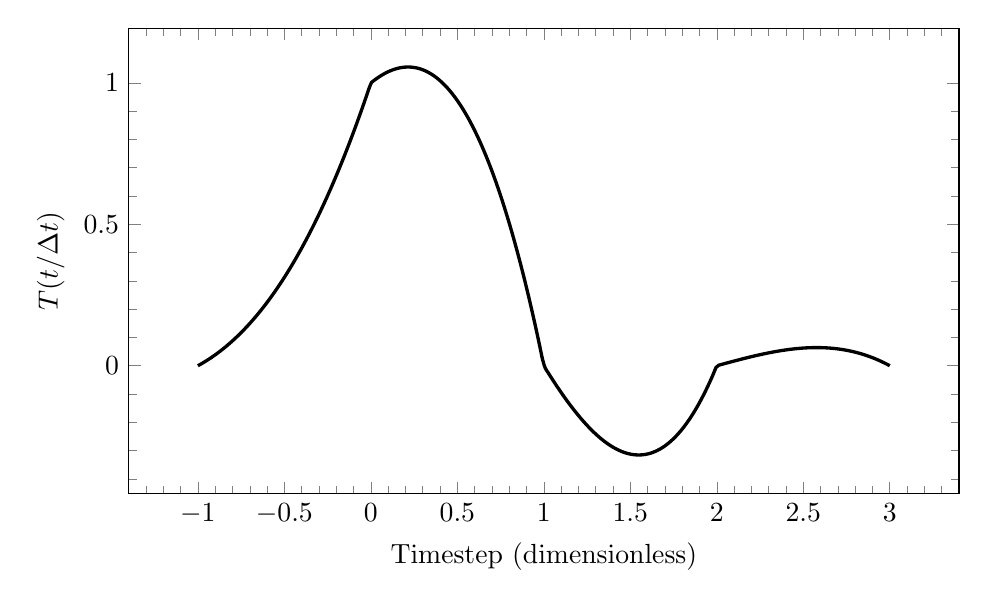
\begin{tikzpicture}[
  declare function = {
    basis(\x) = 
      and(-1 <= \x, \x < 0)*(1+x)*(2+x)*(3+x)/6 +
      and(0  <= \x, \x < 1)*(1-x)*(1+x)*(2+x)/2 +
      and(1  <= \x, \x < 2)*(1-x)*(2-x)*(1+x)/2 + 
      and(2  <= \x, \x < 3)*(1-x)*(2-x)*(3-x)/6 + 
      or(\x <-1, \x > 3)*0;
  }
  ]

  \begin{axis}[width=\columnwidth, height=0.61803398875\columnwidth,
      %xtick={-4, -3, -2, -1},
      minor x tick num={4},
      minor y tick num={4},
      xlabel = Timestep (dimensionless),
      ylabel = {$T(t/\Delta t)$}
      %xticklabels={$-4\Delta t$, $-3\Delta t$, $-2\Delta t$, $-\Delta t$}
  ]
  
  \addplot[very thick, domain=-1:3, smooth, samples=256] {basis(x)};
  \end{axis}
\end{tikzpicture}
